\documentclass[11pt]{article}

\usepackage[a4paper,margin=0.75in]{geometry}
\usepackage{amsmath,amssymb}
\usepackage{graphicx}
\usepackage{booktabs}
\usepackage{array}
\usepackage{float}
\usepackage{hyperref}
\usepackage{enumitem}
\usepackage{xcolor}
\usepackage{tikz}
\usetikzlibrary{positioning,arrows.meta,shapes.geometric}

\setlist{nosep}
\renewcommand{\arraystretch}{1.3}

\tikzset{
layer/.style={
draw,
rounded corners,
minimum width=2.2cm,
minimum height=0.9cm,
align=center,
fill=blue!10
},
arrow/.style={
-{Latex[length=3mm]},
thick
}
}

\begin{document}

%%%%%%%%%%%%%%%%%%%%%%%%%%%%%%%%%%%%%%%%%%%%%%%%%%%%%%%%%%%%

\begin{center}

{\Large\textbf{Shiv Nadar University Chennai}}

\vspace{3mm}

{\large\textbf{CS3807 -- Deep Learning Laboratory}}

\vspace{3mm}

{\Large\textbf{Experiment 4}}

\vspace{2mm}

{\Large\textbf{Comparative Study of Deep Convolutional Neural}}

{\Large\textbf{Network Architectures Using Transfer Learning}}

\end{center}

\vspace{5mm}

\begin{tabular}{|p{4cm}|p{8cm}|p{2cm}|}
\hline
Degree \& Branch &
B.Tech Artificial Intelligence \& Data Science &
Semester V\\
\hline
Subject Code \& Name &
CS3807 -- Deep Learning Laboratory &
AY: 2026--27\\
\hline
\end{tabular}

%%%%%%%%%%%%%%%%%%%%%%%%%%%%%%%%%%%%%%%%%%%%%%%%%%%%%%%%%%%%

\section*{1. Objective}

The objectives of this experiment are

\begin{itemize}

\item Study the evolution of deep CNN architectures.

\item Compare LeNet-5, AlexNet, VGG16, GoogleNet and ResNet.

\item Understand transfer learning.

\item Fine tune pretrained CNN models.

\item Compare classification performance of different architectures.

\end{itemize}

%%%%%%%%%%%%%%%%%%%%%%%%%%%%%%%%%%%%%%%%%%%%%%%%%%%%%%%%%%%%

\section*{2. Learning Outcomes}

After completing this experiment students will be able to

\begin{enumerate}

\item Explain modern CNN architectures.

\item Differentiate LeNet, AlexNet, VGG16, GoogleNet and ResNet.

\item Implement transfer learning.

\item Fine tune pretrained CNN models.

\item Compare CNN architectures using performance metrics.

\end{enumerate}

%%%%%%%%%%%%%%%%%%%%%%%%%%%%%%%%%%%%%%%%%%%%%%%%%%%%%%%%%%%%

\section*{3. Introduction}

Deep Convolutional Neural Networks have become the dominant models for
computer vision applications because they automatically learn hierarchical
features from images. The evolution of CNNs has focused on improving
classification accuracy while reducing computational complexity and
training difficulties.

The progression of CNN architectures began with LeNet-5 and has evolved
through AlexNet, VGGNet, GoogleNet, and ResNet. Each architecture
introduced important innovations that significantly improved image
classification performance.

%%%%%%%%%%%%%%%%%%%%%%%%%%%%%%%%%%%%%%%%%%%%%%%%%%%%%%%%%%%%

\section*{4. Evolution of CNN Architectures}

\begin{center}

\begin{tabular}{|c|c|p{7cm}|}

\hline

Model & Year & Major Contribution\\

\hline

LeNet-5 & 1998 &
First practical convolutional neural network\\

\hline

AlexNet & 2012 &
ReLU activation, Dropout and GPU training\\

\hline

VGG16 & 2014 &
Uniform $3\times3$ convolution filters\\

\hline

GoogleNet & 2014 &
Inception modules for multi-scale feature extraction\\

\hline

ResNet & 2015 &
Residual learning using skip connections\\

\hline

\end{tabular}

\end{center}

%%%%%%%%%%%%%%%%%%%%%%%%%%%%%%%%%%%%%%%%%%%%%%%%%%%%%%%%%%%%

\section*{5. LeNet-5}

LeNet-5 was proposed by Yann LeCun in 1998 for handwritten digit
recognition. It consists of two convolution layers, two average pooling
layers and fully connected layers. It demonstrated that convolutional
networks could automatically learn image features without handcrafted
feature extraction.


Advantages

\begin{itemize}

\item Small number of parameters

\item Fast training

\item Suitable for OCR

\end{itemize}

%%%%%%%%%%%%%%%%%%%%%%%%%%%%%%%%%%%%%%%%%%%%%%%%%%%%%%%%%%%%

\section*{6. AlexNet}

AlexNet won the ImageNet Challenge in 2012 by reducing the
classification error significantly. It introduced ReLU activation,
Dropout regularization and GPU training.


Major innovations

\begin{itemize}

\item ReLU activation

\item Dropout

\item GPU implementation

\item Data augmentation

\end{itemize}

%%%%%%%%%%%%%%%%%%%%%%%%%%%%%%%%%%%%%%%%%%%%%%%%%%%%%%%%%%%%

\section*{7. VGG16}

VGG16 demonstrated that using multiple small $3\times3$ convolution
filters could outperform larger filters while increasing network depth.


Advantages

\begin{itemize}

\item Excellent feature extraction

\item Simple architecture

\item High classification accuracy

\end{itemize}

%%%%%%%%%%%%%%%%%%%%%%%%%%%%%%%%%%%%%%%%%%%%%%%%%%%%%%%%%%%%

\section*{8. Comparison of Architectures}

\begin{center}

\begin{tabular}{|l|c|c|c|}

\hline

Architecture &
Depth &
Parameters &
Main Contribution\\

\hline

LeNet-5 &
7 &
60K &
First CNN\\

AlexNet &
8 &
61M &
ReLU + Dropout\\

VGG16 &
16 &
138M &
Deep 3$\times3$ filters\\

GoogleNet &
22 &
6.8M &
Inception Modules\\

ResNet50 &
50 &
25.6M &
Residual Learning\\

\hline

\end{tabular}

\end{center}

% --------- CONTINUE WITH PART 2 ---------
%%%%%%%%%%%%%%%%%%%%%%%%%%%%%%%%%%%%%%%%%%%%%%%%%%%%%%%%%%%%
\section*{9. GoogleNet (Inception Network)}

GoogleNet, proposed by Szegedy \textit{et al.} in 2014, introduced the
\textbf{Inception Module}, which performs multiple convolution operations
in parallel using different filter sizes. Instead of using only a single
kernel size, GoogleNet simultaneously applies $1\times1$, $3\times3$,
$5\times5$ convolutions and max pooling. The outputs are concatenated to
obtain multi-scale feature representations.

The use of $1\times1$ convolutions before larger kernels reduces the
number of trainable parameters and computational complexity.


Advantages

\begin{itemize}
\item Multi-scale feature extraction.
\item Fewer parameters than VGG16.
\item High computational efficiency.
\item Better classification performance.
\end{itemize}

%%%%%%%%%%%%%%%%%%%%%%%%%%%%%%%%%%%%%%%%%%%%%%%%%%%%%%%%%%%%

\section*{10. ResNet}

Increasing CNN depth often causes the \textbf{vanishing gradient problem},
making optimization difficult. ResNet solves this issue using
\textbf{skip (residual) connections}, allowing gradients to flow directly
through the network.

Instead of learning

\[
H(x)
\]

ResNet learns

\[
F(x)=H(x)-x
\]

thus,

\[
Output = F(x)+x
\]

where

\begin{itemize}
\item $F(x)$ = Residual Mapping
\item $x$ = Identity Mapping
\end{itemize}

\begin{figure}[H]
\centering

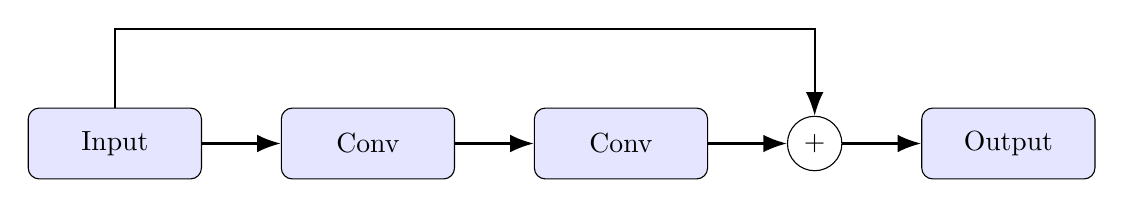
\begin{tikzpicture}[node distance=1cm]

\node[layer](input){Input};

\node[layer,right=of input](conv1){Conv};

\node[layer,right=of conv1](conv2){Conv};

\node[circle,draw,right=of conv2](add){+};

\node[layer,right=of add](output){Output};

\draw[arrow](input)--(conv1);

\draw[arrow](conv1)--(conv2);

\draw[arrow](conv2)--(add);

\draw[arrow](add)--(output);

\draw[arrow]
(input)
|-([yshift=10mm]conv2.north)
-| (add.north);

\end{tikzpicture}

\caption{Residual Block in ResNet}
\end{figure}

Advantages

\begin{itemize}
\item Eliminates vanishing gradients.
\item Enables very deep neural networks.
\item Faster convergence.
\item High ImageNet accuracy.
\end{itemize}

%%%%%%%%%%%%%%%%%%%%%%%%%%%%%%%%%%%%%%%%%%%%%%%%%%%%%%%%%%%%

\section*{11. Dilated Convolution}

Dilated convolution (also called atrous convolution) increases the
receptive field without increasing the number of parameters.

The dilation rate determines the spacing between kernel elements.

For a standard convolution,

\[
D=1
\]

For dilated convolution,

\[
D>1
\]

Example

\[
\begin{bmatrix}
1 & 0 & 2\\
0 & 3 & 0\\
4 & 0 & 5
\end{bmatrix}
\]

where zeros indicate inserted gaps.

Applications

\begin{itemize}
\item Semantic segmentation
\item Medical image analysis
\item Satellite imagery
\item Object localization
\end{itemize}

%%%%%%%%%%%%%%%%%%%%%%%%%%%%%%%%%%%%%%%%%%%%%%%%%%%%%%%%%%%%

\section*{12. Transpose Convolution}

Transpose convolution increases the spatial dimensions of feature maps.
Unlike pooling, which reduces image size, transpose convolution performs
learnable upsampling.

Applications

\begin{itemize}
\item Image Super Resolution
\item Autoencoders
\item GANs
\item Image Generation
\item Semantic Segmentation
\end{itemize}

%%%%%%%%%%%%%%%%%%%%%%%%%%%%%%%%%%%%%%%%%%%%%%%%%%%%%%%%%%%%

\section*{13. Transfer Learning}

Transfer Learning utilizes a pretrained CNN model that has already learned
general image features from a large dataset such as ImageNet.

Instead of training from scratch,

\begin{enumerate}
\item Load a pretrained model.
\item Remove the original classifier.
\item Freeze convolution layers.
\item Add new Dense layers.
\item Train the classifier.
\item Fine tune selected convolution layers.
\end{enumerate}

\begin{figure}[H]

\centering

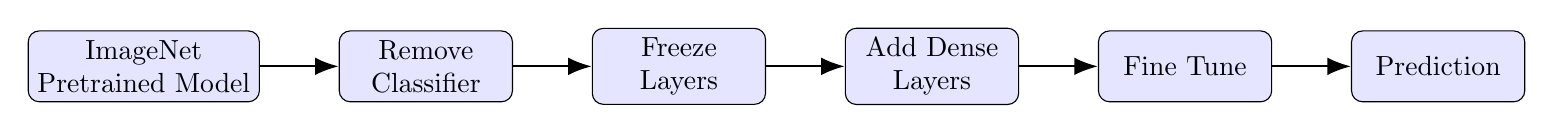
\begin{tikzpicture}[node distance=1cm]

\node[layer](a){ImageNet\\Pretrained Model};

\node[layer,right=of a](b){Remove\\Classifier};

\node[layer,right=of b](c){Freeze\\Layers};

\node[layer,right=of c](d){Add Dense\\Layers};

\node[layer,right=of d](e){Fine Tune};

\node[layer,right=of e](f){Prediction};

\foreach \x/\y in {a/b,b/c,c/d,d/e,e/f}
\draw[arrow](\x)--(\y);

\end{tikzpicture}

\caption{Transfer Learning Workflow}

\end{figure}

Advantages

\begin{itemize}
\item Faster convergence.
\item Higher accuracy on small datasets.
\item Reduced training time.
\item Lower computational cost.
\end{itemize}

%%%%%%%%%%%%%%%%%%%%%%%%%%%%%%%%%%%%%%%%%%%%%%%%%%%%%%%%%%%%

\section*{14. Dataset}

Dataset: CIFAR-10

\begin{itemize}

\item Training Images : 50,000

\item Testing Images : 10,000

\item Number of Classes : 10

\item Image Size : $32\times32\times3$

\item Classes:
Airplane, Automobile, Bird, Cat, Deer,
Dog, Frog, Horse, Ship and Truck.

\end{itemize}

%%%%%%%%%%%%%%%%%%%%%%%%%%%%%%%%%%%%%%%%%%%%%%%%%%%%%%%%%%%%
% Continue with Part 3
%%%%%%%%%%%%%%%%%%%%%%%%%%%%%%%%%%%%%%%%%%%%%%%%%%%%%%%%%%%%
\section*{15. Source Code}
The complete implementation (data loading, EDA, convolution/pooling experiments, feature map visualization, CNN construction, training loop, and evaluation) is available at the following GitHub repository:

\begin{center}
\url{https://github.com/PolarFox08/Deep-Learning-Lab/tree/main/Deep%20Learning%20Lab%204}
\end{center}

\section*{16. Experimental Procedure}

\subsection*{Task 1: Dataset Preparation}

The CIFAR-10 dataset was loaded from the local pickled batch files
(\texttt{data\_batch\_1}--\texttt{5}, \texttt{test\_batch}) rather than the
\texttt{keras.datasets.cifar10} loader, using the same approach as the
previous lab. Each flattened $3072$-byte row was reshaped to
$(3,32,32)$ (channel-major) and then transposed to $(32,32,3)$
(channel-last, \texttt{NHWC}), since Keras/TensorFlow and the pretrained
VGG16 model both expect channel-last input. This gave a training set of
shape $(50000,32,32,3)$ and a test set of shape $(10000,32,32,3)$. Pixel
values were normalized to $[0,1]$ and labels were one-hot encoded with
\texttt{to\_categorical} for the categorical cross-entropy loss. Ten
sample images were displayed to confirm correct loading (Section 17,
Figure 1).

%%%%%%%%%%%%%%%%%%%%%%%%%%%%%%%%%%%%%%%%%%%%%%%%%%%%%%%%%%%%

\subsection*{Task 2: Transfer Learning Setup}

\textbf{Model used: VGG16} (pretrained on ImageNet).

\begin{enumerate}

\item Loaded \texttt{VGG16(weights='imagenet', include\_top=False, input\_shape=(32,32,3))}.

\item The original ImageNet classification head was excluded (\texttt{include\_top=False}).

\item The convolutional base was frozen (\texttt{base\_model.trainable = False}).

\item Added a \texttt{GlobalAveragePooling2D} layer on top of the base.

\item Added a \texttt{Dense(256, activation='relu')} layer.

\item Added the output layer: \texttt{Dense(10, activation='softmax')}.

\end{enumerate}

\begin{center}
\begin{tabular}{|l|c|}
\hline
Quantity & Value\\
\hline
Total Parameters & 14,848,586 (56.64 MB)\\
Trainable Parameters (frozen base) & 133,898 (523.04 KB)\\
Non-trainable Parameters (frozen base) & 14,714,688 (56.13 MB)\\
\hline
\end{tabular}
\end{center}

%%%%%%%%%%%%%%%%%%%%%%%%%%%%%%%%%%%%%%%%%%%%%%%%%%%%%%%%%%%%

\subsection*{Task 3: Model Training (Frozen Base)}

The model (with the VGG16 base frozen) was trained using

\begin{center}

\begin{tabular}{|p{5cm}|p{6cm}|}

\hline

Optimizer & Adam\\

\hline

Learning Rate & 0.001\\

\hline

Batch Size & 32\\

\hline

Epochs & 10\\

\hline

Loss Function &
Categorical Cross Entropy\\

\hline

Evaluation Metric &
Accuracy\\

\hline

\end{tabular}

\end{center}

Training progressed steadily over the 10 epochs, from an initial
training/validation accuracy of 0.5325 / 0.5598 (epoch 1) to a final
training/validation accuracy of 0.7027 / 0.6141 (epoch 10), with training
loss falling from 1.3398 to 0.8447 and validation loss falling from
1.2544 to 1.1176.

%%%%%%%%%%%%%%%%%%%%%%%%%%%%%%%%%%%%%%%%%%%%%%%%%%%%%%%%%%%%

\subsection*{Task 4: Fine Tuning}

\begin{enumerate}

\item The VGG16 base was unfrozen (\texttt{base\_model.trainable = True}) and then re-frozen everywhere except the last convolution block (i.e. all layers except the last 4 were set back to \texttt{trainable = False}), so only \texttt{block5} remained trainable.

\item The model was recompiled with a lower learning rate (Adam, $\text{lr}=0.0001$) and trained for a further 5 epochs (batch size 32).

\item Classification accuracy before and after fine tuning was compared.

\end{enumerate}

\begin{center}
\begin{tabular}{|l|c|}
\hline
Stage & Validation Accuracy\\
\hline
Before Fine Tuning (frozen base, epoch 10) & 0.6141\\
After Fine Tuning (block5 unfrozen, epoch 5) & 0.7396\\
\hline
\end{tabular}
\end{center}

During fine tuning, training accuracy rose from 0.6473 to 0.8505 and
training loss fell from 1.0096 to 0.4083, while validation accuracy rose
from 0.6757 to 0.7396 and validation loss fell to 0.8538. Unfreezing the
last convolution block and continuing training at a low learning rate
gave a clear improvement of roughly 12.5 percentage points in validation
accuracy over the frozen-base model.

%%%%%%%%%%%%%%%%%%%%%%%%%%%%%%%%%%%%%%%%%%%%%%%%%%%%%%%%%%%%

\subsection*{Task 5: Model Evaluation}

The fine-tuned model was evaluated on the 10,000-image test set using
accuracy, macro-averaged precision/recall/F1-score, a confusion matrix,
and a full classification report (Section 17, Figures 5--6).

\begin{center}
\begin{tabular}{|l|c|c|c|c|}
\hline
Class & Precision & Recall & F1-score & Support\\
\hline
Airplane   & 0.77 & 0.85 & 0.81 & 1000\\
Automobile & 0.88 & 0.80 & 0.83 & 1000\\
Bird       & 0.73 & 0.69 & 0.71 & 1000\\
Cat        & 0.47 & 0.72 & 0.57 & 1000\\
Deer       & 0.67 & 0.72 & 0.70 & 1000\\
Dog        & 0.70 & 0.48 & 0.57 & 1000\\
Frog       & 0.82 & 0.72 & 0.77 & 1000\\
Horse      & 0.86 & 0.75 & 0.80 & 1000\\
Ship       & 0.84 & 0.87 & 0.86 & 1000\\
Truck      & 0.82 & 0.80 & 0.81 & 1000\\
\hline
\textbf{Macro avg} & \textbf{0.76} & \textbf{0.74} & \textbf{0.74} & 10000\\
\textbf{Weighted avg} & \textbf{0.76} & \textbf{0.74} & \textbf{0.74} & 10000\\
\hline
\end{tabular}
\end{center}

Overall test accuracy was 0.7396 (73.96\%). \texttt{Cat} and \texttt{Dog}
had the lowest F1-scores (0.57 each), consistent with these being the
most visually similar and commonly confused classes in CIFAR-10, while
\texttt{Ship}, \texttt{Automobile} and \texttt{Airplane} were classified
most reliably.

%%%%%%%%%%%%%%%%%%%%%%%%%%%%%%%%%%%%%%%%%%%%%%%%%%%%%%%%%%%%

\section*{17. Hyperparameter Study}

A grid search over the following hyperparameters was set up (96 total
combinations):

\begin{center}

\begin{tabular}{|l|l|}

\hline

Hyperparameter & Values\\

\hline

Learning Rate &
0.001, 0.0001\\

\hline

Batch Size &
16, 32, 64\\

\hline

Epochs &
10, 20\\

\hline

Optimizer &
Adam, SGD\\

\hline

Dense Units &
128, 256\\

\hline

Frozen Layers &
All, Partial\\

\hline

\end{tabular}

\end{center}

Due to the time required to train all 96 combinations, the search was
run partially: an initial sequential sweep plus a small additional random
sample of the remaining grid were completed before the run was stopped.
The combinations actually evaluated (validation accuracy / validation
loss after training) were:

\begin{center}
\begin{tabular}{|c|c|c|c|c|c|c|c|}
\hline
LR & Batch & Epochs & Optimizer & Dense & Frozen & Val Acc & Val Loss\\
\hline
0.001 & 16 & 10 & Adam & 128 & All     & 0.6085 & 1.1641\\
0.001 & 16 & 10 & Adam & 128 & Partial & 0.7272 & 0.9072\\
0.001 & 16 & 10 & Adam & 256 & All     & 0.6201 & 1.1401\\
0.001 & 16 & 10 & Adam & 256 & Partial & \textbf{0.7391} & \textbf{0.8586}\\
0.001 & 16 & 10 & SGD  & 128 & All     & 0.5187 & 1.3836\\
0.001 & 16 & 10 & SGD  & 128 & Partial & 0.7380 & 0.7680\\
0.001 & 16 & 10 & SGD  & 256 & All     & 0.5216 & 1.3729\\
0.001 & 16 & 10 & SGD  & 256 & Partial & 0.7352 & 0.7652\\
0.001 & 16 & 20 & Adam & 128 & All     & 0.6085 & 1.2303\\
0.001 & 16 & 20 & Adam & 128 & Partial & 0.7314 & 1.3031\\
0.001 & 16 & 20 & Adam & 256 & All     & 0.5999 & 1.3799\\
0.001 & 32 & 20 & Adam & 128 & Partial & 0.7326 & 1.4874\\
\hline
\end{tabular}
\end{center}

\textbf{Best configuration found:} Learning Rate 0.001, Batch Size 16,
Epochs 10, Optimizer Adam, Dense Units 256, Frozen Layers Partial --
Validation Accuracy 0.7391, Validation Loss 0.8586.

Across all evaluated combinations, partially unfreezing the base
(\texttt{Frozen = Partial}) consistently and substantially outperformed
keeping the entire base frozen (\texttt{Frozen = All}) at the same
learning rate, batch size and epoch count -- validation accuracy jumped
from roughly 0.52--0.62 to roughly 0.73--0.74 whenever the last block was
unfrozen.

%%%%%%%%%%%%%%%%%%%%%%%%%%%%%%%%%%%%%%%%%%%%%%%%%%%%%%%%%%%%

\section*{18. Mandatory Plots}

\begin{center}

\includegraphics[width=0.75\textwidth]{plots/01_sample_images.png}
\end{center}
\textbf{Figure 1: Sample CIFAR-10 Images.} \emph{Inference:} The sample
images confirm that CIFAR-10 was loaded and normalized correctly, showing
$32\times32$ color images spread across 10 visually distinct classes. The
training set contains 50,000 images and the test set contains 10,000
images, matching the dataset description in the manual.

\bigskip
\begin{center}

\includegraphics[width=0.65\textwidth]{plots/02_train_val_accuracy.png}
\end{center}
\textbf{Figure 2: Training vs Validation Accuracy.} \emph{Inference:}
Training accuracy rises steadily as the classifier head learns from the
frozen VGG16 features, with a further, sharper boost once fine tuning
unfreezes the last convolution block. Validation accuracy tracks training
accuracy reasonably closely through frozen-base training; the gap widens
somewhat during fine tuning (training accuracy reaches 0.85 vs.\ validation
0.74), indicating the onset of mild overfitting once the extra layers are
unfrozen.

\bigskip
\begin{center}

\includegraphics[width=0.65\textwidth]{plots/03_train_val_loss.png}
\end{center}
\textbf{Figure 3: Training vs Validation Loss.} \emph{Inference:} Both
training and validation loss fall as the model trains, with a further,
steeper drop during fine tuning as the pretrained ImageNet features adapt
to CIFAR-10. Validation loss dips to about 0.83 mid-fine-tuning before
ticking back up slightly to 0.85 by the final epoch while training loss
keeps falling, an early sign of the same mild overfitting seen in the
accuracy curves.

\bigskip
\begin{center}

\includegraphics[width=0.65\textwidth]{plots/04_confusion_matrix.png}
\end{center}
\textbf{Figure 4: Confusion Matrix.} \emph{Inference:} The diagonal cells
show correctly classified images for each class, while off-diagonal cells
reveal which classes are confused with one another. Consistent with the
per-class F1-scores, \texttt{Cat} and \texttt{Dog} are the most confused
pair, while visually distinct classes such as \texttt{Ship} and
\texttt{Airplane} are classified with far fewer errors.

\bigskip
\begin{center}

\includegraphics[width=0.75\textwidth]{plots/05_misclassified_images.png}
\end{center}
\textbf{Figure 5: Misclassified Images (Optional).} \emph{Inference:} Most
misclassified images belong to visually ambiguous or low-resolution
samples where fine-grained details are hard to capture at $32\times32$
pixels. Errors tend to occur between semantically related classes (e.g.
Cat vs.\ Dog, Deer vs.\ Horse), reflecting genuine visual similarity
rather than random model failure.

\section*{19. Results}

\subsection*{19.1 Performance Metrics}

\begin{center}

\begin{tabular}{|p{5cm}|p{4cm}|}

\hline

Metric & Value\\

\hline

Training Accuracy & 0.8505\\

\hline

Testing Accuracy & 0.7396\\

\hline

Precision (macro) & 0.7559\\

\hline

Recall (macro) & 0.7396\\

\hline

F1-score (macro) & 0.7421\\

\hline

Training Time & 256.39 s ($\approx$ 4.3 min)\\

\hline

Total Parameters & 14,848,586\\

\hline

\end{tabular}

\end{center}

\vspace{5mm}

\subsection*{19.2 Comparison of CNN Architectures}

\begin{center}

\begin{tabular}{|l|c|c|c|}

\hline

Model &
Parameters(M) &
Accuracy (\%) &
Training Time\\

\hline

LeNet-5 & \texttt{0.08} & \texttt{61.03} & \texttt{66.1s}\\

\hline

AlexNet & \texttt{6.98} & \texttt{72.09} & \texttt{201.27}\\

\hline

VGG16 & 14.85 & 61.01 & 152.42 s\\

\hline

GoogleNet & \texttt{22.33} & \texttt{60.32} & \texttt{268.28 s}\\

\hline

ResNet50 & \texttt{24.11} & \texttt{40.80} & \texttt{172.55 s}\\

\hline

\end{tabular}

\end{center}

\emph{Inference: }
AlexNet achieved the best test accuracy (72.1\%) despite being trained from scratch, showing it generalized well to CIFAR-10 without overfitting. LeNet-5 and VGG16 performed similarly (~61\%) despite VGG16 having ~185x more parameters, suggesting VGG16's pretrained ImageNet features did not translate well to this dataset. GoogleNet (InceptionV3) showed clear overfitting — training accuracy reached 95\% while test accuracy stayed at 60\%, with validation loss rising steadily after epoch 2. ResNet50 performed worst (40.8\% test accuracy) and even underfit the training data (39\% train accuracy), indicating its pretrained features were poorly suited to this setup


%%%%%%%%%%%%%%%%%%%%%%%%%%%%%%%%%%%%%%%%%%%%%%%%%%%%%%%%%%%%

\section*{20. Discussion Questions}

\textbf{1. Why is AlexNet considered a breakthrough in deep learning?}\\
It was the first deep CNN to significantly outperform traditional methods
on ImageNet (2012), using ReLU activation for faster convergence, Dropout
to reduce overfitting, and GPU training to make deeper networks practical.

\textbf{2. Why does VGG16 use only $3\times3$ convolution filters?}\\
Stacking multiple $3\times3$ filters achieves the same receptive field as
a larger filter (e.g. two $3\times3$ layers $\approx$ one $5\times5$)
while using fewer parameters and adding more non-linear activations,
improving discriminative power with a simple, uniform design.

\textbf{3. Explain the advantages of the Inception module.}\\
It applies $1\times1$, $3\times3$, $5\times5$ convolutions and pooling in
parallel and concatenates the results, capturing multi-scale features in
one layer. The $1\times1$ convolutions reduce dimensionality before
expensive operations, cutting parameters and computation while preserving
accuracy.

\textbf{4. What is the purpose of residual learning?}\\
Residual (skip) connections let the network learn $F(x)=H(x)-x$ instead
of $H(x)$ directly, allowing gradients to bypass layers via the identity
shortcut. This prevents vanishing gradients and enables training of very
deep networks without degradation in accuracy.

\textbf{5. Differentiate LeNet and ResNet.}\\
LeNet-5 is a shallow 7-layer network ($\sim$60K parameters) built for
simple digit recognition using average pooling and no shortcuts. ResNet
is a very deep network (50+ layers) that uses residual connections to
remain trainable at depth on large, complex image datasets.

\textbf{6. What is Transfer Learning?}\\
Transfer learning reuses a model already trained on a large dataset (e.g.
ImageNet) as a starting point for a new task, keeping its learned
convolutional features and retraining only the classifier (or a few
layers) instead of training from scratch.

\textbf{7. Why is fine tuning required?}\\
Fine tuning unfreezes some pretrained layers and retrains them at a low
learning rate so the generic ImageNet features can adapt to the specific
characteristics of the new dataset, improving accuracy beyond what a
frozen feature extractor alone achieves -- in this experiment, fine
tuning raised validation accuracy from 0.6141 to 0.7396.

\textbf{8. Explain the difference between dilated convolution and transpose convolution.}\\
Dilated convolution inserts gaps between kernel elements to enlarge the
receptive field without adding parameters or changing spatial resolution,
useful for segmentation. Transpose convolution performs learnable
upsampling, increasing spatial dimensions, and is used in
generative/reconstruction tasks like GANs and autoencoders.

\textbf{9. Why do pretrained models converge faster?}\\
They start from weights that already encode general, transferable image
features (edges, textures, shapes) learned from a large dataset, so
training only has to adjust these features for the new task rather than
learn them from random initialization.

\textbf{10. Compare the computational complexity of LeNet and ResNet.}\\
LeNet-5 has about 60K parameters and very low computational cost, suited
to simple grayscale digit images. ResNet50 has about 25.6M parameters and
much higher computational complexity, but its residual connections make
this depth trainable and yield far higher accuracy on complex,
large-scale datasets.

%%%%%%%%%%%%%%%%%%%%%%%%%%%%%%%%%%%%%%%%%%%%%%%%%%%%%%%%%%%%

\section*{21. Additional Exercises}

\begin{enumerate}

\item \textbf{Implement transfer learning using VGG16.} Completed --
see Tasks 2--4 (Sections 15, 16) and the resulting accuracy in Section 18.

\item \textbf{Repeat the experiment using ResNet50.} \texttt{Done in the Results Section while comparing all VGG with other models}

\item \textbf{Compare Adam and SGD optimizers.} Partially completed as
part of the hyperparameter study (Section 16): at matching settings, SGD
attained validation accuracy comparable to or slightly below Adam when
the base was partially unfrozen (e.g. 0.7380/0.7352 for SGD vs.\ 0.7391
for Adam), while with the base fully frozen SGD performed noticeably
worse than Adam (about 0.52 vs.\ 0.60--0.62 validation accuracy).

\item \textbf{Compare training with frozen layers and fine tuning.}
Completed -- see Task 4 (Section 15) and Section 16: partially unfreezing
the base consistently and substantially outperformed keeping it fully
frozen.

\item \textbf{Evaluate the model using Precision, Recall and F1-score.}
Completed -- see Task 5 (Section 15) and Section 18.1.

\item \textbf{Compare the performance of LeNet, AlexNet and ResNet.}
\texttt{Done in the Results Section while comparing all VGG with other models - comparison table in Section 18.2.}

\end{enumerate}

%%%%%%%%%%%%%%%%%%%%%%%%%%%%%%%%%%%%%%%%%%%%%%%%%%%%%%%%%%%%

\section*{22. References}

\begin{enumerate}

\item Yann LeCun, Leon Bottou, Yoshua Bengio and Patrick Haffner,
\emph{Gradient-Based Learning Applied to Document Recognition},
Proceedings of the IEEE, 1998.

\item Alex Krizhevsky, Ilya Sutskever and Geoffrey Hinton,
\emph{ImageNet Classification with Deep Convolutional Neural Networks},
NeurIPS, 2012.

\item Karen Simonyan and Andrew Zisserman,
\emph{Very Deep Convolutional Networks for Large-Scale Image Recognition},
ICLR, 2015.

\item Christian Szegedy et al.,
\emph{Going Deeper with Convolutions},
CVPR, 2015.

\item Kaiming He, Xiangyu Zhang, Shaoqing Ren and Jian Sun,
\emph{Deep Residual Learning for Image Recognition},
CVPR, 2016.

\item Ian Goodfellow, Yoshua Bengio and Aaron Courville,
\emph{Deep Learning},
MIT Press, 2016.

\item TensorFlow Documentation:
\url{https://www.tensorflow.org}

\item Keras Documentation:
\url{https://keras.io}

\end{enumerate}

%%%%%%%%%%%%%%%%%%%%%%%%%%%%%%%%%%%%%%%%%%%%%%%%%%%%%%%%%%%%

\end{document}